\section{NEXT: A HPXe TPC}
%%%

%%%%%%%%%%
\begin{figure}
\centering
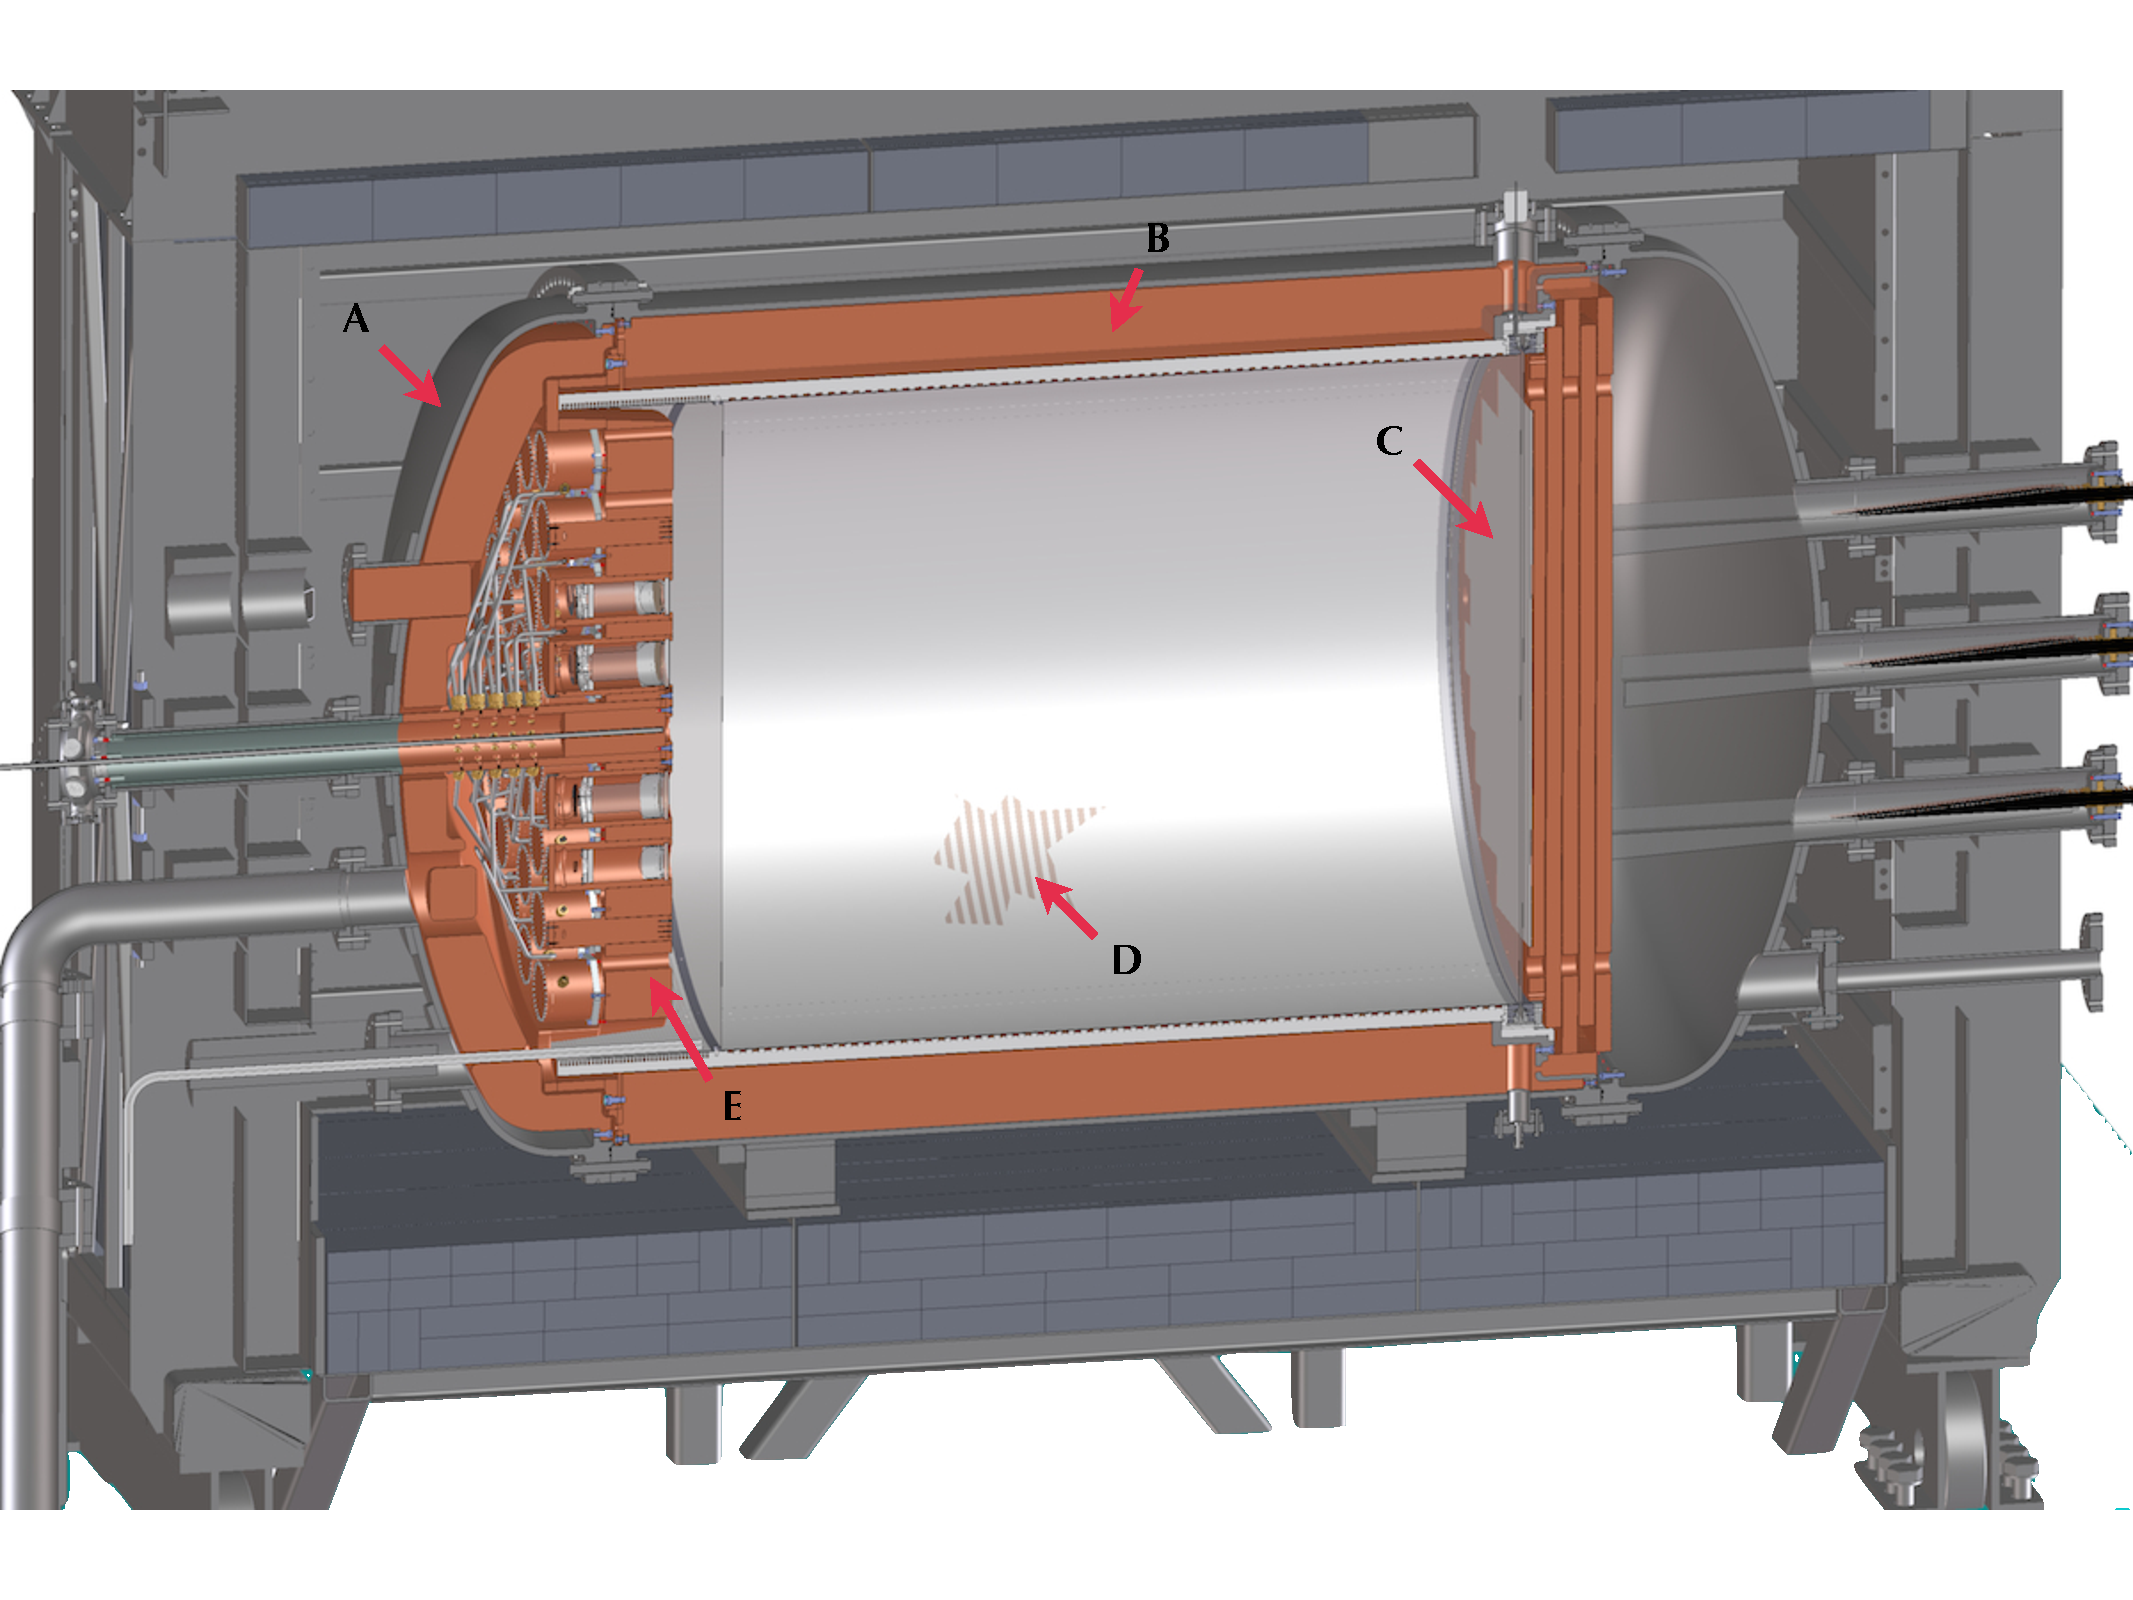
\includegraphics[width=0.9\textwidth]{img/Next100.pdf}
\caption{A cross-section drawing of the NEXT-100 detector. The pressure vessel (A) is made of stainless steel Grade 316Ti, and its dimensions are 130~cm inner diameter, 222~cm length and 1~cm thick walls, for a total mass of 1\,200 kg. The inner copper shield (B) is made of ultra-pure copper bars and is 12~cm thick, with a total mass of 9\,000 kg. The time projection chamber (D) includes the field cage, cathode, EL grids and HV penetrators. The light tube is made of thin teflon sheets coated with TPB (a wavelength shifter). The energy plane (E) is made of 60 PMTs housed in copper enclosures. The tracking plane (C) is made of MPPCs arranged into 8$\times$8 boards.} \label{fig.NEXT100}
\end{figure}
%%%%%%%%%%

The \emph{Neutrino Experiment with a Xenon TPC} (NEXT) \cite{Gomez-Cadenas:2013lta} will search for the neutrinoless double beta decay of \XE\ using a high-pressure xenon gas time projection chamber. The design of the NEXT-100 detector (Figure \ref{fig.NEXT100}) is optimised for energy resolution by using proportional electroluminescent (EL) amplification of the ionisation signal. The detection process involves the use of the prompt scintillation light from the gas as start-of-event time, and the drift of the ionisation charge to the anode by means of an electric field ($\sim0.3$ kV/cm at 15 bar) where secondary EL scintillation is produced in the region defined by two highly transparent meshes, between which there is a field of $\sim20$ kV/cm at 15 bar. The detection of EL light provides an energy measurement using photomultipliers (PMTs) located behind the cathode (the \emph{energy plane}) as well as tracking through its detection a few mm away from production at the anode, via a dense array of silicon photomultipliers (the \emph{tracking plane}).

\begin{figure}
\centering
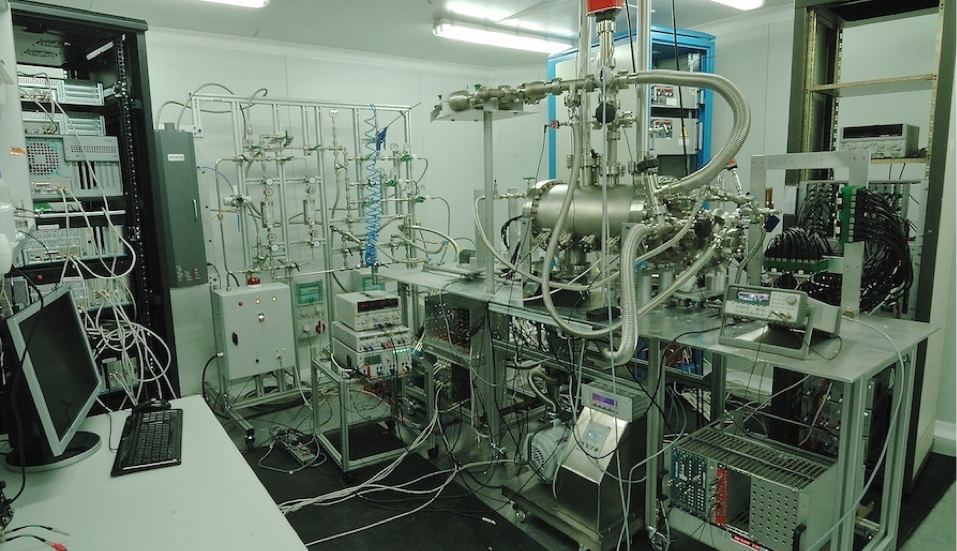
\includegraphics[width=0.9\textwidth]{img/DemoSetup.png}
\caption{\small The NEXT-DEMO setup at IFIC (Valencia, Spain).} \label{fig.DEMO}
\end{figure}

The R\&D phase of the experiment was carried out with the large-scale prototypes NEXT-DEMO (shown in Figure \ref{fig.DEMO}) and NEXT-DBDM. The prototypes have measured excellent energy resolution, extrapolating to 0.5--0.7 \% FWHM at \Qbb\  \cite{Alvarez:2012xda,Alvarez:2012kua,Lorca:2014sra}. 

%%%%%
\begin{figure}
\centering
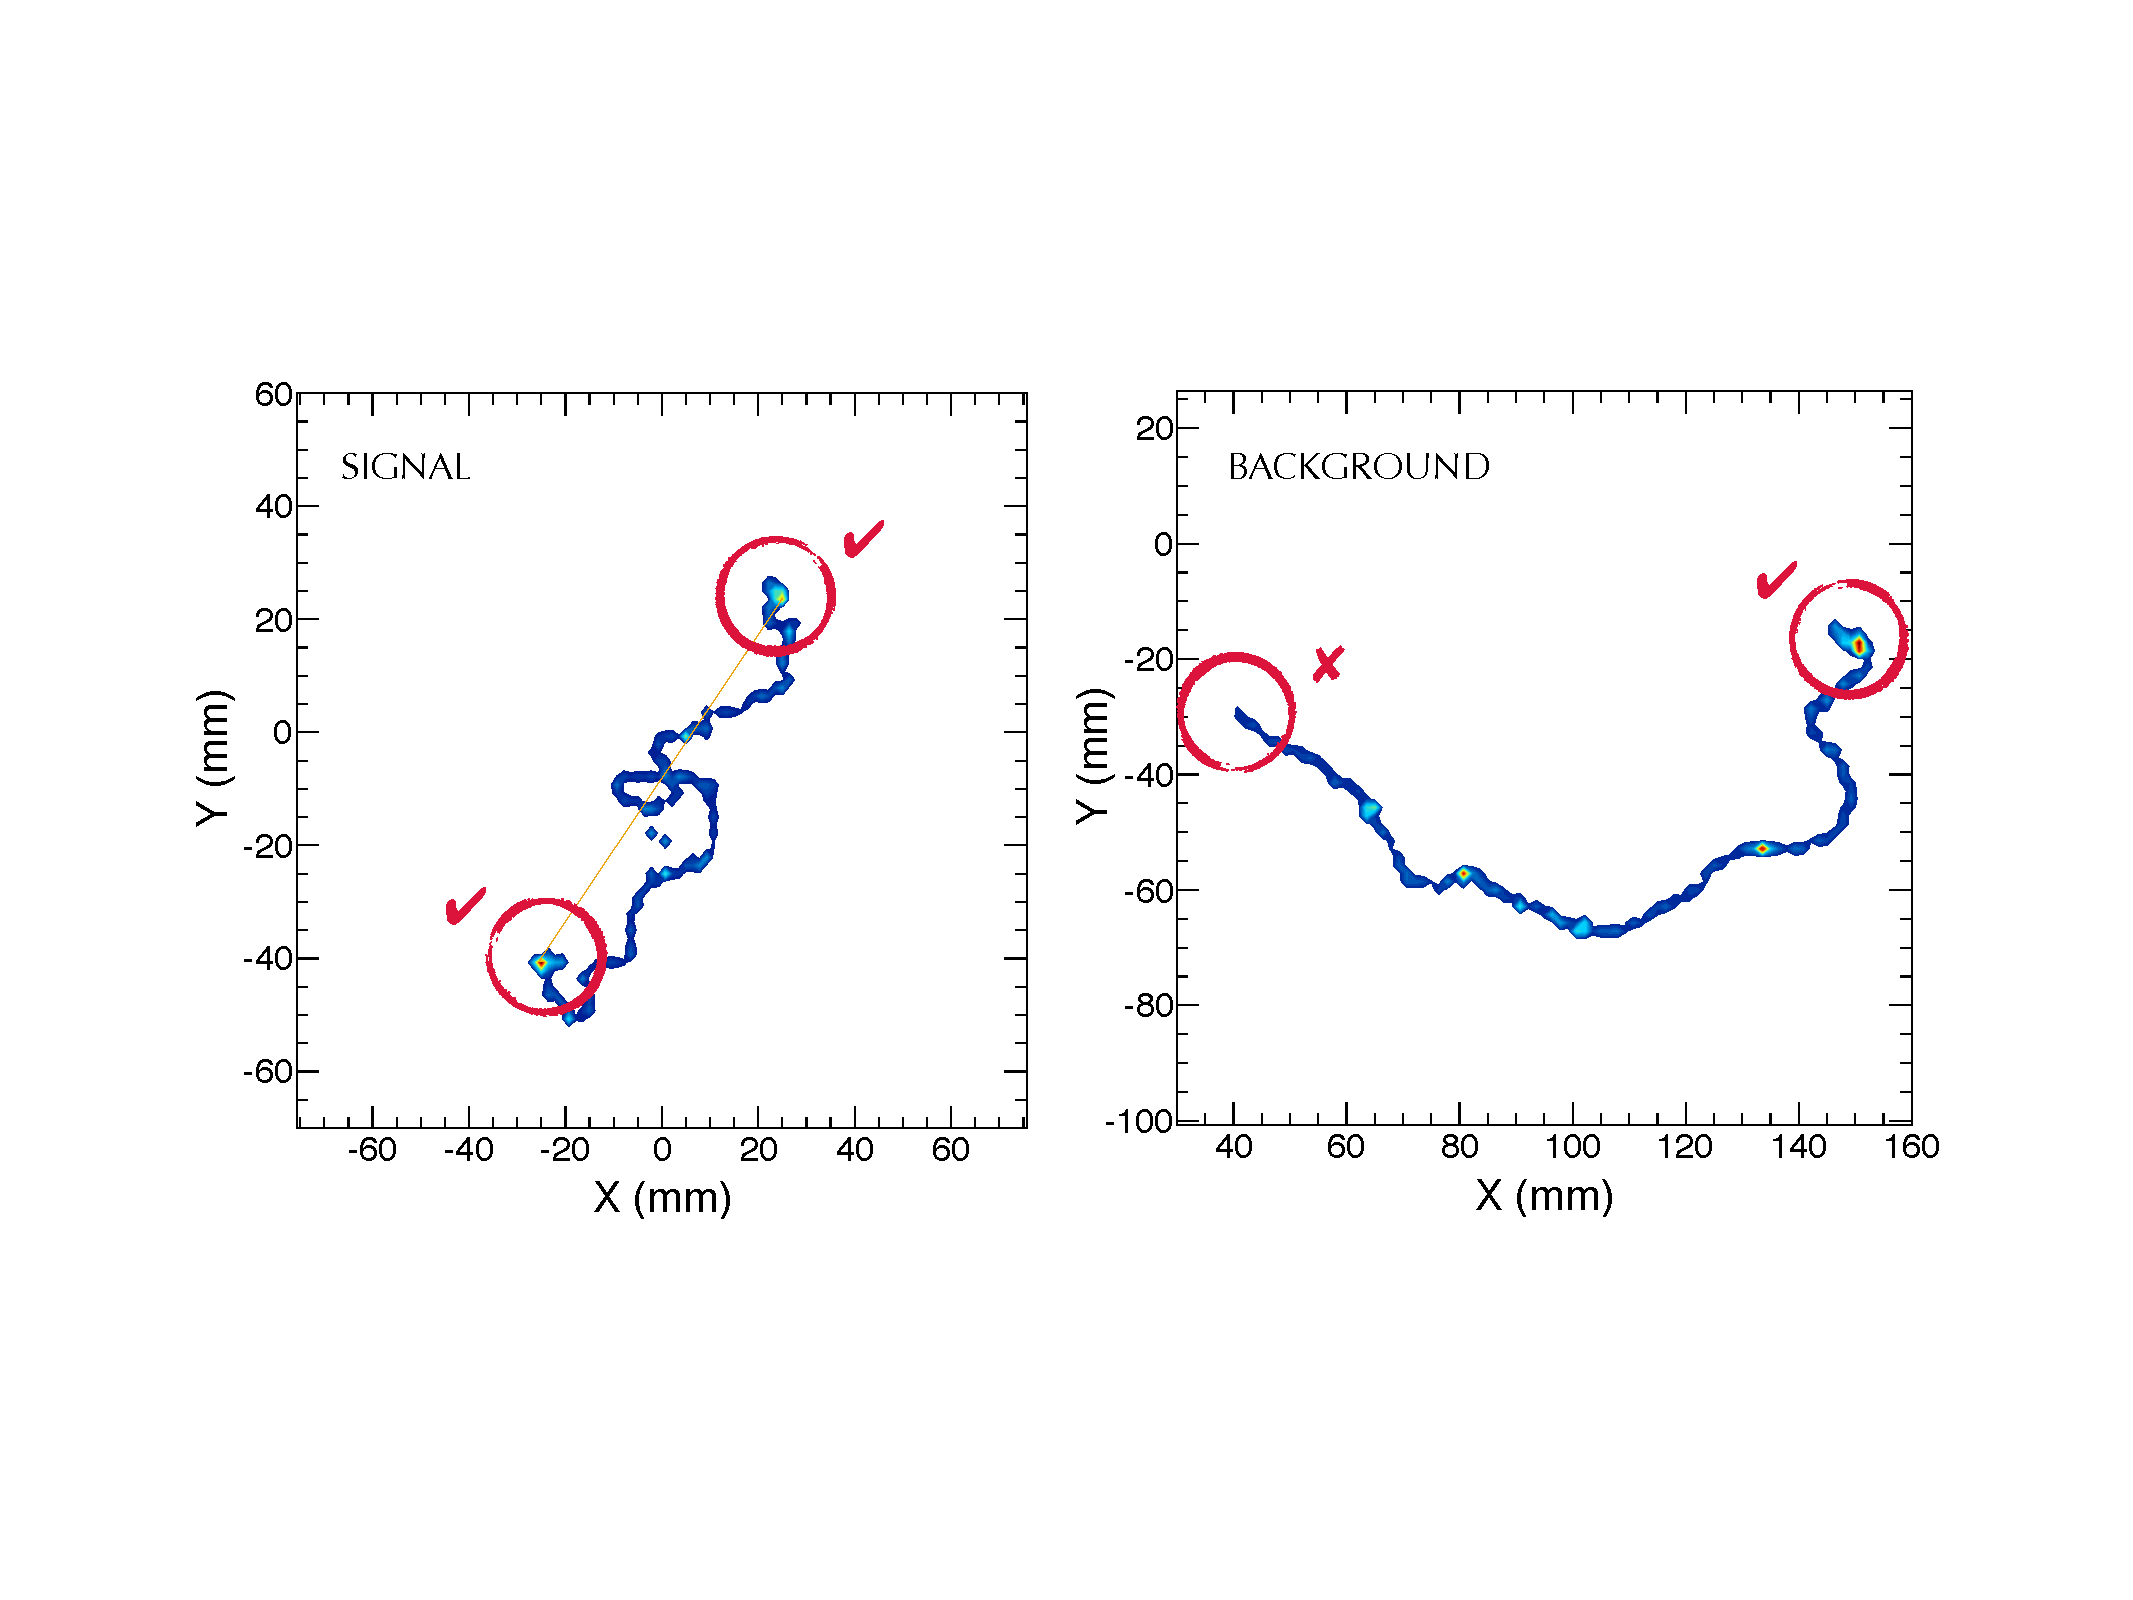
\includegraphics[width= 0.9\textwidth]{img/TrackSignature.pdf}
\caption{Monte Carlo simulation of a signal (\bbonu) event (left) and a  background event (right) in xenon gas at 15~bar. The color codes energy deposition in the gas. The signal consist of two electrons emitted from a common vertex, and thus it features large energy depositions  (blobs) at both ends of the track. Background event are, typically, single-electron tracks (produced by photoelectric of Compton interactions of high energy gammas emitted by \BI\ or \TL\ isotopes), and thus feature only one blob.} \label{fig.ETRK2}
\end{figure}
%%%%%

%%%%%
\begin{figure}
\centering
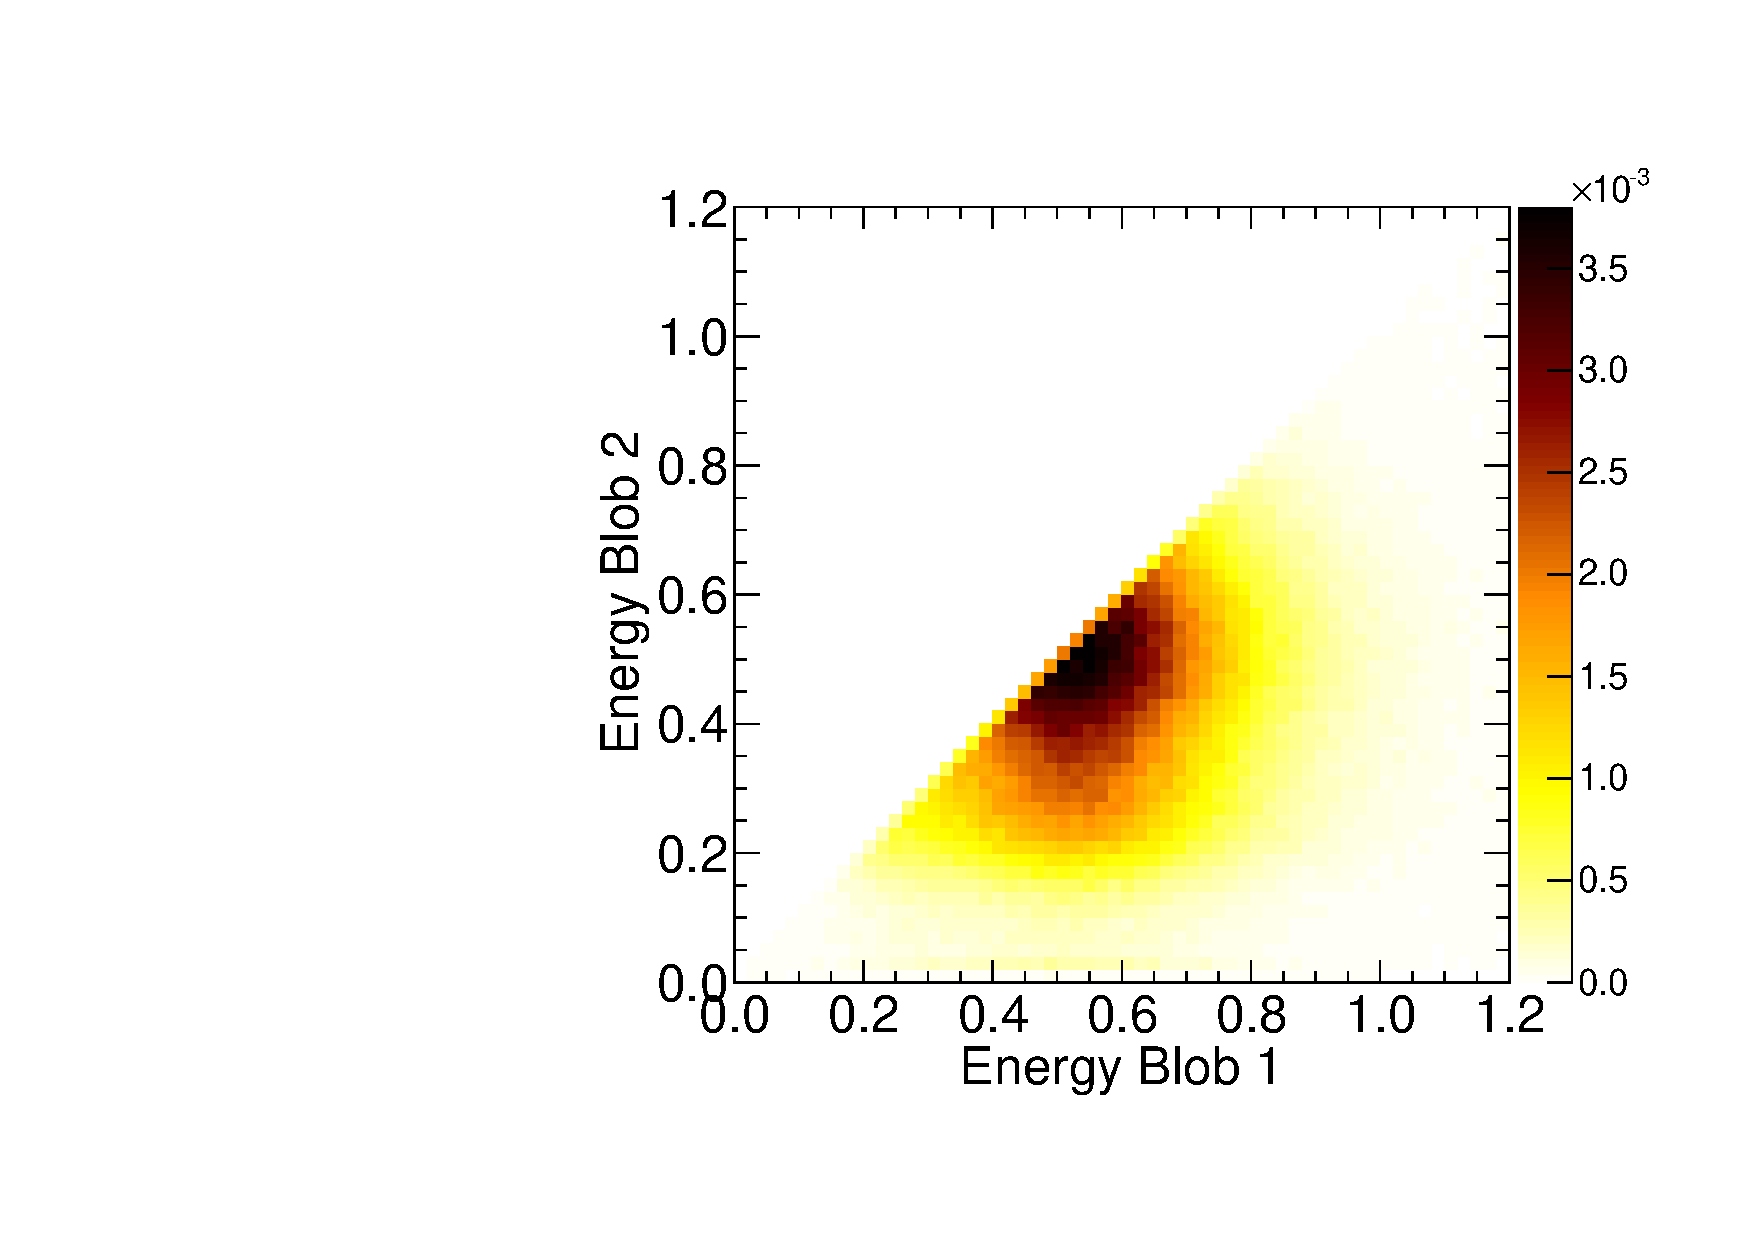
\includegraphics[width=0.45\textwidth]{img/EnergyBlobsSignal.pdf}
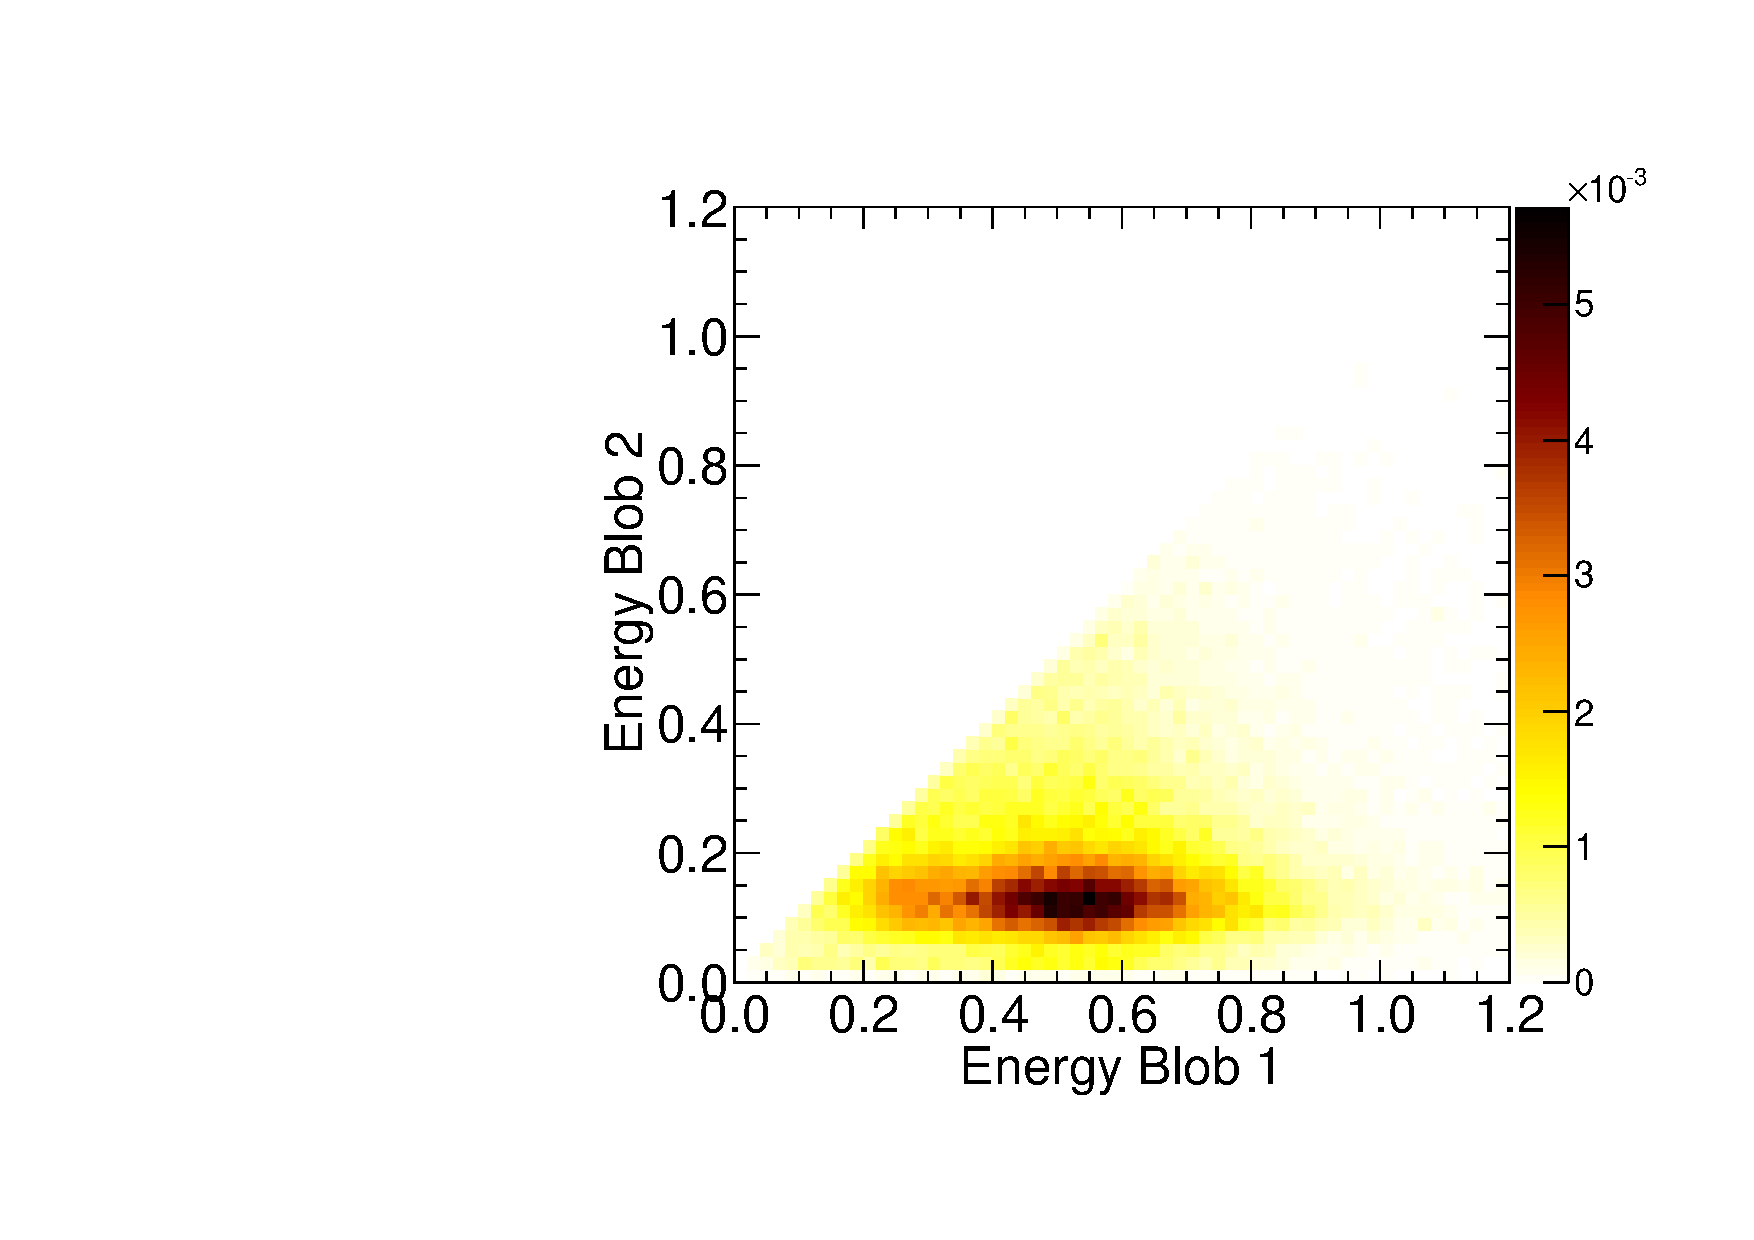
\includegraphics[width=0.45\textwidth]{img/EnergyBlobsTl208.pdf}
\caption{Probability distribution of signal (left) and background (right) events in terms of the energies of the end-of-track blobs. The blob labelled as `1' corresponds to the more energetic one, whereas `blob 2' corresponds to the less energetic of the two. In a signal event, the blobs have, in average, the same energy. In a background event, blob 1 has the same energy than a signal event while the energy of blob 2 is very small.} \label{fig.BLOBS}
\end{figure}
%%%%%

In addition of excellent energy reconstruction, NEXT has a topological signature, not available in most \bbonu\ detectors. 
Double beta decay events leave a distinctive topological signature in HPXe: a continuous track with larger energy depositions (\emph{blobs}) at both ends due to the Bragg-like peaks in the d$E$/d$x$ of the stopping electrons (figure \ref{fig.ETRK2}, top left). In contrast, background electrons are produced by Compton or photoelectric interactions, and are characterised by a single blob and, often, by a satellite cluster corresponding to the emission of 30-keV fluorescence X-rays by xenon (figure \ref{fig.ETRK2}).
Reconstruction of this topology using the tracking plane provides a powerful means of background rejection, as can be observed in Figure \ref{fig.BLOBS}. 

\subsection{NEXT background model}

 The major sources of background can be found in the 
radioactive contaminants in detector materials, in particular \BI\ and \TL\ isotopes.
The decay of \BI\ emits a number of de-excitation gammas with energies above 2.3 MeV. The gamma line at 2447 keV, of intensity 1.57\%, is very close to the $Q$-value of \XE. The gamma lines above \Qbb\ have low intensity and their contribution is negligible. 
The decay of \TL\ emits a de-excitation photon of 2614 keV with a 100\% intensity. The Compton edge of this gamma is at 2382 keV, well below \Qbb. However, the scattered gamma can interact and produce other electron tracks close enough to the initial Compton electron so they are reconstructed as a single object falling in the energy region of interest (ROI). Photoelectric electrons are produced above the ROI but can loose energy via bremsstrahlung and populate the window, in case the emitted photons escape out of the detector. Pair-creation events are not able to produce single-track events in the ROI. 

Radon constitutes also dangerous source of background due to the radioactive isotopes $^{222}$Rn (half-life of 3.8\,d) from the $^{238}$U chain and $^{220}$Rn (half-life of 55\,s) from the $^{232}$Th chain. As a gas, it diffuses into the air and can enter the detector. \BI\ is a decay product of $^{222}$Rn, and \TL\ a decay product of $^{220}$Rn. In both cases, radon undergoes an alpha decay into polonium, producing a positively charged ion which is drifted towards the cathode by the electric field of the TPC.  As a consequence, $^{214}$Bi and $^{208}$Tl contaminations can be assumed to be deposited on the cathode surface. Radon may be eliminated from the TPC gas mixture by recirculation through appropriate filters. There are also ways to suppress radon in the volume defined by the shielding. 

A detailed discussion of the NEXT background model can be found in \cite{Nebot-Guinot:2014raa}.

The excellent resolution of NEXT (0.5-0.7 \% FWHM), and the combination of a low radioactive budget with a topological signature (which yields an expected background rate of $5 \times 10^{-4} \ckky$), will allow the NEXT-100 detector to reach a sensitivity to the \bbonu\ period of $\Tonu > 7 \times 10^{25}$~yr for a exposure of 300 kg$\cdot$yr. This translates into a \mbb\ sensitivity range as low as $[67-187]$~meV, depending on the NME.

The detector is expected to start data taking in 2017. Currently, the first phase of the experiment, called NEW is being commissioned at the Canfranc Underground Laboratory (LSC), in Spain, and will start data taking later in 2015.
 

\section{BEXT: A HPXe TPC Operating in a Magnetic Field}

\subsection{Economy of Scale in a HPXe TPC}

\begin{figure}
\centering
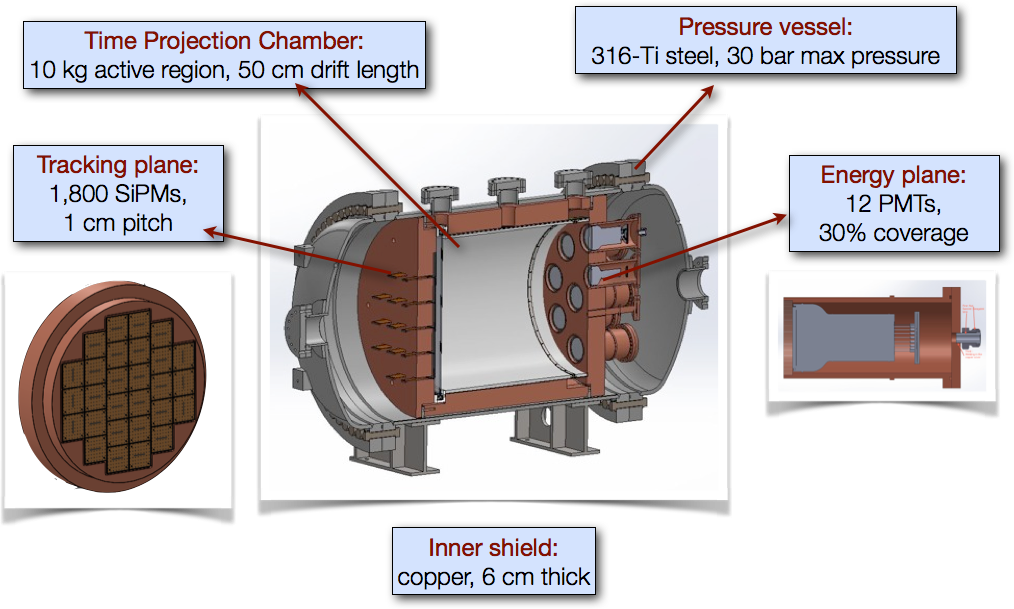
\includegraphics[width=0.9\textwidth]{img/NEW.png}
\caption{\small The NEW detector, currently being commissioned at the LSC (Canfranc, Spain).} \label{fig.NEW}
\end{figure}

The NEW detector, shown in Figure \ref{fig.NEW}, is the first phase of the NEXT experiment. The fiducial volume is a cylinder of 50 cm diameter and 60 cm length. The fiducial mass, at a pressure of 15 bar is 10 kg. The tracking plane has about 2,000 SiPMs, while the energy plane deploys 12 PMTs.

The fiducial volume of NEXT-100 (Figure \ref{fig.NEXT100}) is a cylinder of 110 cm diameter and 1200 cm length. The fiducial mass, at a pressure of 15 bar is $\sim$100 (98.5) kg. The tracking plane has about 9,000 SiPMs, while the energy plane deploys 60 PMTs.

The comparison between the first and the second phase of the NEXT experiment reveals clearly that a HPXe TPC benefits from the so-called {\em economy of scale} law, which in turn is a simple consequence of the fact that an HPXe is an homogeneous detector with a target mass ($M$) proportional to the fiducial volume (FV). If one approximates the FV by a cube of length $L$, then, doubling $L$ ($L \rightarrow 2 L$) results in multiplying the surface by 4 ($4 L^2$) and the volume by 8 ($8 L^3$). On the other hand, both the sensors need to instrument the apparatus and the backgrounds are roughly proportional to the detector surface, while the target mass (and therefore the signal) is proportional to the detector volume. Therefore the ratio signal to background (S/B) (and the cost of instrumentation versus the cost of the isotope) decreases linearly with $L$. In a detector without economy of scale (e.g. a detector built by repeating modules, such as the Germanium arrays), neither S/B nor the relative cost of instrumenting the system improve as the target mass increases. 

Indeed, both NEW and NEXT-100 are cylinders of near 1:1 aspect ratio (the diameter of the cylinder, $D$ is only slightly larger than the cylinder length $L$). Then, denoting $D_{NEXT}, L_{NEXT}, M_{NEXT}$~to the diameter, length and fiducial mass of NEXT-100 and $D_{NEW}, L_{NEW}, M_{NEW}$~to the diameter, length and fiducial mass of NEW, we find that doubling the NEW diameter (plus a 10\%), $D_{NEXT} = 1.1 \times 2 \times D_{NEW}$, and doubling the NEW length $L_{NEXT} = 2 \times L_{NEW}$, one increases the fiducial mass by one order of magnitude $M_{NEXT} = 10 \times M_{NEW}$, and the number of sensors by a factor 2 (plus a 10\%). 

The recipe to increase the fiducial mass to one ton is, then, appears straight forward: repeating the recipe:
we find that doubling the NEXT-100 diameter (plus a 10\%), $D_{BEXT} = 1.1 \times 2 \times D_{NEXT} \sim 2.4$~ m, and doubling the NEXT length $L_{BEXT} = 2 \times L_{NEXT} =2.4$~m, one increases the fiducial mass to almost one ton $M_{BEXT} = 954$~kg. To instrument the detector one would need about 45,000 SiPMs in the tracking plane (and about 250 PMTs in the energy plane). The naive ``economy of scale'' extrapolation law would predict that such a detector (if instrumented with the same sensors and materials than its predecessor and operating in the same environment) would have roughly a factor 2 less background events per year in the ROI.

\subsection{Operation in a magnetic field}
On the other hand, operation inside an intense magnetic field excludes the use of conventional PMTs, which must be replaced by sensors capable of providing a similar performance, to guarantee the excellent energy resolution characteristic of an HPXe.

Fortunately, a solution exists, already with today's technology. During the last five years, SiPMs have improved their performance in three crucial aspects: a) voltage operation uniformity; b) gain uniformity; and c) dark current.  
For example, SENSL manufactures large area SiPMs ($3 \times 3$~mm$^2$), capable of operating within 125 mV of the nominal voltage, with very small (< 0.5\%) gain spread and few ($\sim 2$) dark counts per photoelectron and micro-second. (REFERENCE?). This opens the possibility that the PMT energy plane is replace by an array of large area SiPMs. 

On the other hand, as will be discussed with detail in section XX, the additional separation power between signal and background attainable with a magnetic field deteriorates with pressure. In our studies, the optimal pressure is found to be 5 bar, but 10 bar provides an acceptable performance. Decreasing the operating pressure, on the other hand, requires an increase in the detector dimensions. Increasing both the diameter and the length to 3 m,
$D_{BEXT} = 3$~m, $L_{BEXT} = 3$~m, one obtains a fiducial mass of 1.2 tons. 

The studies discussed in section XX, also show that the separation between signal and background improves with the point resolution that can be achieved when reconstructing the electrons. Point resolution, in turn, depends of the diffusion in the electron drift and of sensor pitch. In pure xenon, diffusion is large, with typical values of 10 mm (for lateral diffusion) and about 5 mm (for longitudinal diffusion) after a typical drift of 1 m. However, as demonstrated recently by the NEXT collaboration (REF), the addition of very small quantities of a suitable additive (for example 0.1 \% of CO$_2$) reduces both the lateral and longitudinal dimensions to $\sim$ 1--2 mm, while having essentially no impact in the energy resolution. Therefore, BEXT will need to operate with such an additive. 

The SiPM pitch in the tracking plane of NEXT-100 is 10 mm (the sensors themselves are squares of 1 mm$^2$~surface). The minimum point resolution that is achieved in such a configuration is $10/\sqrt(12) = \sim 3$~mm (in practice the resolution is better, since the light emitted in the EL region is shared by more than one pixel, and thus one can reconstruct the position using a weighted procedure such as barycenter) which is much better than the resolution introduced by diffusion. On the other hand, in BEXT the resolution due to diffusion can be reduced to about 1--2 mm. Reducing the tracking plane pitch to 5 mm would result in a minimum resolution of 1.5 mm ($5/\sqrt(12)$). In practice light-sharing may provide a point resolution of 1--2 mm even with the larger pitch. The number of SiPMs needed for the BEXT tracking plane if the pitch is kept at 10 mm will be about 70 k, and about 280 k if the pitch is reduced to 5 mm. On the other hand, manufacturing a large quantity (e.g. 300 k) of SIPMs at very moderate costs (e.g. 3 \$/piece) appears feasible already today, resulting in a reasonable cost for the BEXT tracking sensors ($\sim 1$ M \$).  

The SiPMs making up the energy plane will have a surface of 3 mm$^2$, which appear as a good compromise between sensor area (which must be maximized to increase light collection) and dark current (which is proportional to the area of the sensor and must be kept within a reasonable value). The sensors will be located at a pitch of 10 mm, and Winston cone of outer radius 10 mm and inner radius 3 mm will focus the light in the sensors. Therefore, about 70 k pieces will be needed, at a cost that will probably not exceed 350 k\$. 

\subsection{BEXT conceptual design parameters}
The parameters of BEXT are summarized in Table \ref{tab.BEXT}. As will be shown in section XX the optimal performance for a pressure of 10 bar is achieved with a magnetic field of 0.5--0.7 Tesla. 
\begin{table}[htdp]
\caption{Parameters of BEXT}
\begin{center}
\begin{tabular}{|c|c|}
Parameter & Value \\
Magnetic field & Solenoidal, 0.5--0.7 Tesla \\
Operating pressure (bar) & 10 \\
Fiducial Volume & Cylinder of 21.1 m$^3$\\
Radius (m) & 1.5 \\
Drift Length (m) & 3 \\
Fiducial Mass (ton) & 1.2 \\
Tracking Plane & \\
Size of SiPMs (mm$^2$) & 1 \\
Pitch & 5 mm \\
Number of SiPMs & 280,000 \\
Energy Plane & \\
Size of SiPMs (mm$^2$) & 9 \\
Pitch & 10 mm \\
Number of SiPMs & 70,000 \\
\end{tabular}
\end{center}
\label{tab.BEXT}
\end{table}%
  



%As will be discussed with great detail later in this paper, the use of a magnetic field adds an extra handle to the topological signature, illustrated in Figure \ref{fig.KF}. 
%In the presence of a uniform external magnetic field $B$, charged particles spiral around the field lines in circular motion with radius $r = p_T/eB$, where $p_T$~ is the momentum of the electron transverse to the direction of the field and $e$~ is the electron charge. In the absence of multiple scattering, a single energetic electron produces a  single spiral with radius indicative of its momentum, and a double-electron track with the same energy will produce two spirals each with much less momentum and originating from a common vertex. This information can be used to provide an additional way of separating single-electrons arising from background processes from double electrons produced in \bbonu\ decays.
%However, in a dense medium such as xenon at high pressure, multiple scattering enters the picture, altering the electron trajectories and making it harder to distinguish signal from backgrounds. 
% 
% Figure \ref{fig.KF} illustrates the discussion. The top-left panel shows two electrons emitted in a \bbonu\ decay in the absence of magnetic field. Notice that the vertex where both electrons originated cannot be easily measured due to multiple scattering. However, the presence of two electrons is revealed by the two blobs at the end of the tracks (regions with higher density of hits and energy deposition, which originate when each one of the electron ranges out). Instead, the top-right panel shows a single background electron, which originates inside the detector when a photon, emitted by the decay of the isotope \BI\ enters the chamber and suffers a photoelectric interaction. Notice that the single electron only displays one blob in one of the vertexes. 
%
%When a sufficiently intense magnetic field is added, the separation between single and double electrons is strongly enhanced. The bottom-left panel shows again two electrons emitted in a \bbonu\ decay, turning in a magnetic field of 0.5 Tesla. The trajectory ``remembers'' that which would be followed in the absence of multiple scattering  (two helices originating from a common vertex). The bottom-right panel shows a single background electron turning in a 0.5 T magnetic field, following a single helix. This information can be used to enhance signal-background separation (see section XXX) {\em only if} a reasonable point-resolution (few mm at most) is achieved in the measurement of the track coordinates. To achieve such resolution, one needs to add to the xenon an additive capable of reducing diffusion while preserving the excellent energy resolution of characteristic of an EL TPC. The NEXT collaboration has studied several potential additives such as TMA (Diego paper), CH4 and O2. 
%   
% 
% The current (estimated) rejection factor for NEXT-100 is 0.5 counts per ton and keV in a year. If a resolution of \Qbb\ of 0.5 \% FWHM is confirmed in the large detector as we expect, this translates into 5 counts per ton in the ROI. The addition of a magnetic field may yield a value of 0.5-1 counts per ton in the ROI, thus allowing the HPXe technology to operate in the ton regime without being background limited. 
%
%
%
%


 


